\documentclass{article}
\usepackage{booktabs}
\usepackage{adjustbox}
\usepackage{float}
\usepackage{listings}

\lstset{frame=tb,
  language=Java,
  aboveskip=3mm,
  belowskip=3mm,
  showstringspaces=false,
  columns=flexible,
  basicstyle={\small\ttfamily},
  numbers=none,
  numberstyle=\tiny\color{gray},
  keywordstyle=\color{blue},
  commentstyle=\color{dkgreen},
  stringstyle=\color{mauve},
  breaklines=true,
  breakatwhitespace=true,
  tabsize=3
}


\graphicspath{{/Users/naveen/Desktop/workspace/Stevens FA/FE570/project/images}}

\begin{document}

\section{Liquidity measure}

\section{Intraday volatility}

Volatility is the tendency for prices to change unexpectedly. Prices change in response to new information about values and in response to the demands of impatient traders for liquidity. Fundamental volatility and Trading volatility are two types of volatility at the microscale. \\

Seventeen different exchanges are represented in the Reuters tick data, among which the top four exchanges by trades—ADF, NAX, DEX, and PSE—are selected for the volatility study.


\begin{figure}[H]
\centering
\begin{adjustbox}{max width=\textwidth}
    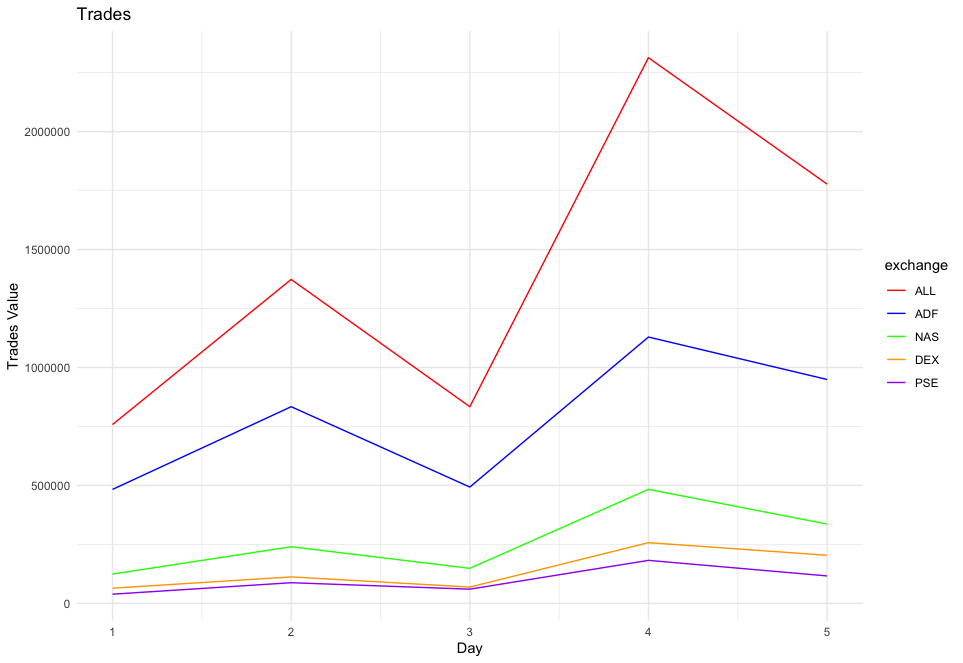
\includegraphics[width=0.8\textwidth]{plot_vol_exchanges.png}
\end{adjustbox}
\caption{Volume across exchanges}
\label{fig:vol_across_exchanges}
\end{figure}

\subsection{Roll model}

The trade price $p_t = m_t + \epsilon_t$ has two components: \\

i) the efficient price $m_t$ and \\

ii) trading noise contribution $\epsilon_t$. \\

Roll model volatility of the increments of the efficient price $\sigma_{u}^2 =\gamma_0 + 2\gamma_1$ \\

$\sigma_{day} = \sqrt{n_{trades} * \sigma_u}$ \\

In the formula $\sigma_{u}^2 =\gamma_0 + 2\gamma_1$, the second term $2\gamma_1$ is negative and subtracts the trading activity contribution from the total volatility. \\

We obtained the fundamental volatility of the stock price $\sigma_{ann} = \frac{\sigma_u}{\overline{S}} \times \sqrt{n_{trades}} \times \sqrt{252}$ \\

The total volatility is obtained by replacing $\sigma_u^2$ with $\gamma_0=var(\Delta p_t)$, the total price volatility. This gives \\

$\sigma_{ann}^{total} = \frac{\sqrt\gamma_u}{\overline{S}} \times \sqrt{n_{trades}} \times \sqrt{252}$ \\


Autocorrelation at lag 1 suggests a short-term dependency between consecutive differenced price values. For lags beyond 1, the autocorrelation values are within the confidence bounds, implying no statistically significant autocorrelation. The pattern in consistent across all five days.

\begin{figure}[H]
\centering
\begin{adjustbox}{max width=\textwidth}
    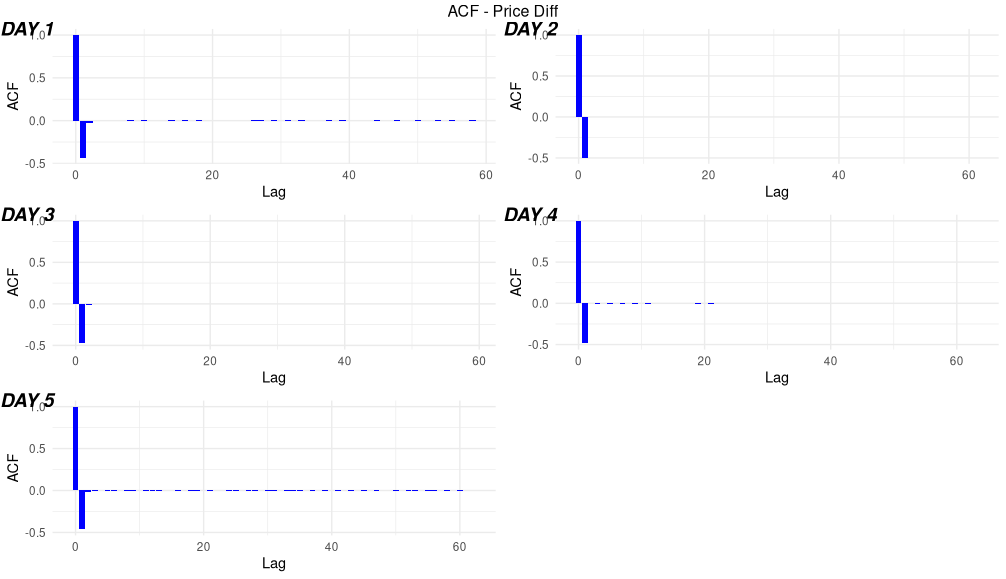
\includegraphics[width=0.8\textwidth]{acf_price_diff.png}
\end{adjustbox}
\caption{Autocorrelation function (ACF) of price differences.}
\label{fig:acf_price_diff}
\end{figure}

The ACF of trade signs shows a slow, gradual decay over the lags, suggesting a persistent autocorrelation in the trade signs.


\begin{figure}[H]
\centering
\begin{adjustbox}{max width=\textwidth}
    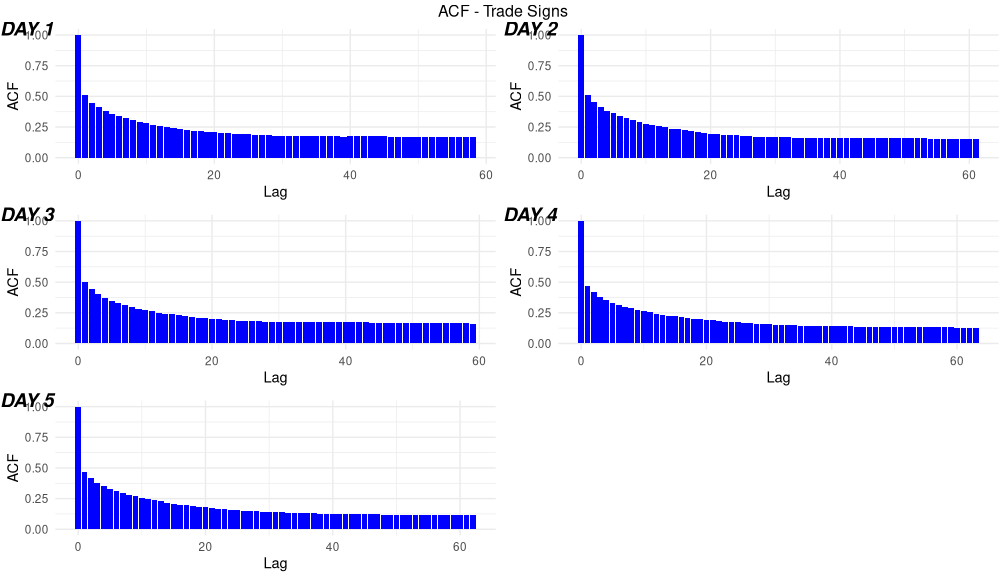
\includegraphics[width=0.8\textwidth]{acf_trade_signs.png}
\end{adjustbox}
\caption{Autocorrelation function (ACF) of trade signs.}
\label{fig:acf_trade_signs}
\end{figure}

For most days, the mid prices closely track the trade prices, indicating a relatively efficient market with minimal divergence between the actual trades and the theoretical mid prices. Sudden spikes in the trade price (red line) suggest high volatility during specific periods.

\begin{figure}[H]
\centering
\begin{adjustbox}{max width=\textwidth}
    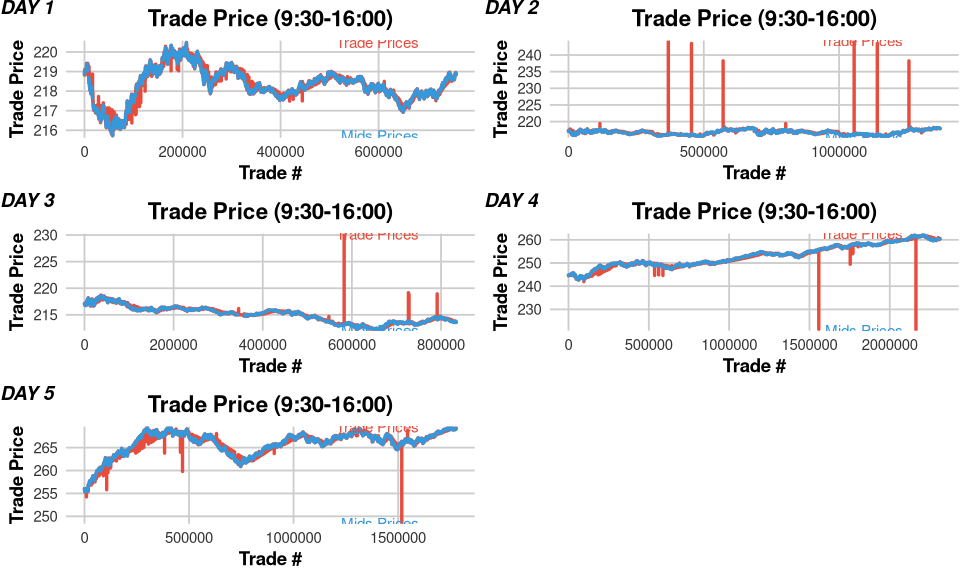
\includegraphics[width=0.8\textwidth]{price_plot_alldays.png}
\end{adjustbox}
\caption{Price plot over all days.}
\label{fig:price_plot_alldays}
\end{figure}

Across all days, most trades have relatively low volumes (a consistent baseline). However, sporadic spikes in trade size suggest periods of high trading activity or large block trades. The volume baseline remains relatively constant across the observed days, with no major shifts in trading patterns except for the spikes. Spikes may indicate either large institutional trades or block trades, reaction to news or market events during speicifc times of the day.


\begin{figure}[H]
\centering
\begin{adjustbox}{max width=\textwidth}
    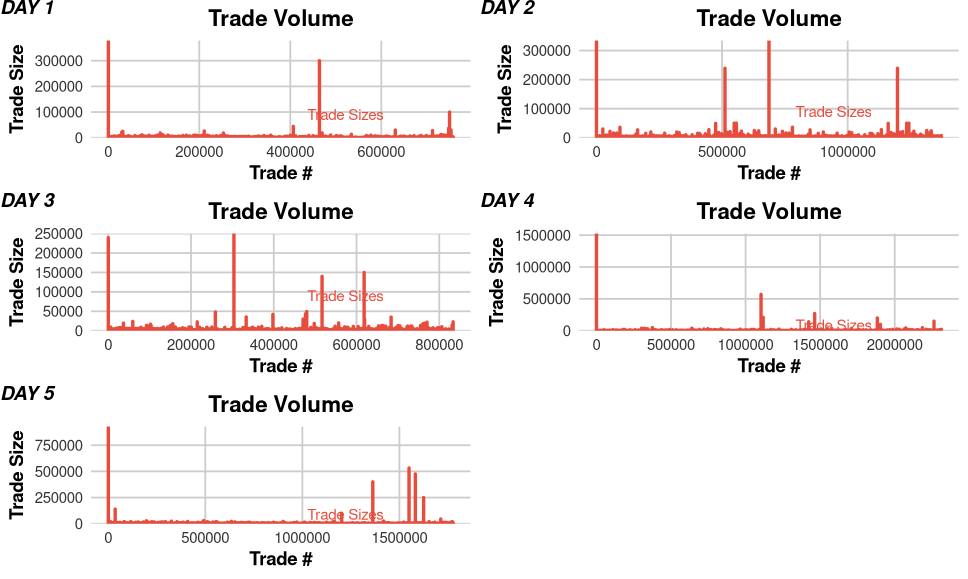
\includegraphics[width=0.8\textwidth]{volume_plot_alldays.png}
\end{adjustbox}
\caption{Volume plot over all days.}
\label{fig:volume_plot_alldays}
\end{figure}

The red line (representing "ALL") generally shows the highest roll values across all days, indicating that the combined market volume or activity across all exchanges is consistently the highest.

There is a dip in roll values for Day 3 across all exchanges, suggesting reduced market activity or lower trading volumes.

By Day 5, all exchanges (ADF, NAS, DEX, PSE) converge to similar roll values, reflecting consistent trading behavior.

A notable drop on Day 3 might indicate a day of lower market participation, possibly due to external events or lack of significant trading catalysts.

On Day 5, roll values across exchanges align, suggesting synchronized trading activity across markets.The convergence of roll values  across exchanges by Day 5 indicates increased market synchronization, likely due to alignment in trading strategies or external factors driving uniform behavior.


\begin{figure}[H]
\centering
\begin{adjustbox}{max width=\textwidth}
    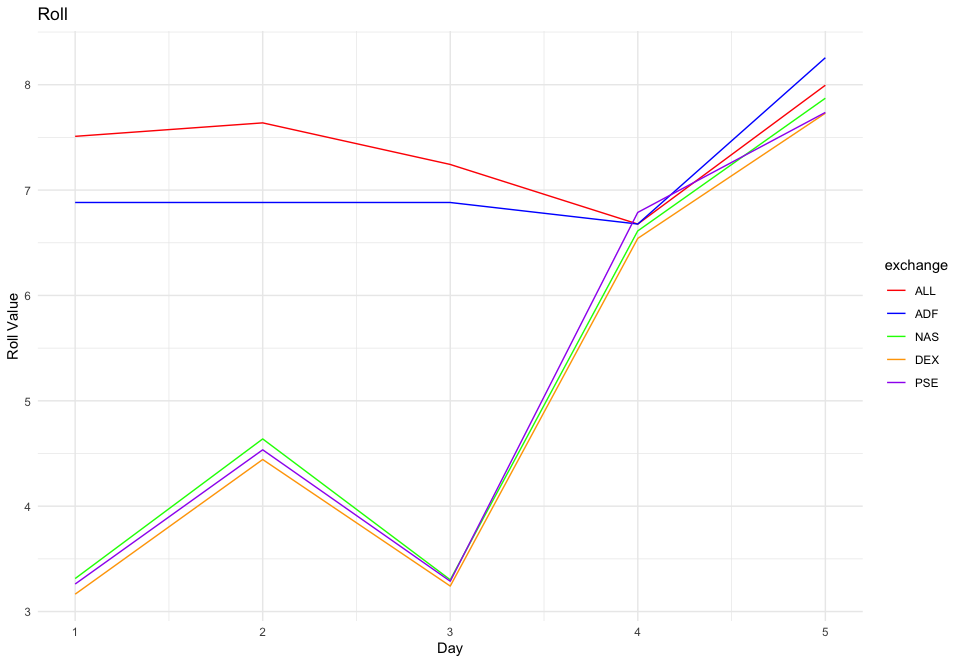
\includegraphics[width=0.8\textwidth]{roll_exchanges.png}
\end{adjustbox}
\caption{$\sigma_{day}^{roll}$ across exchanges}
\label{fig:roll_vol_exhcnage}
\end{figure}


\subsubsection{Roll model estimate - across different exchanges}

Roll model parameters $\gamma_0$ $\gamma_1$ $\sigma^2_u$ $\sigma_{ann}$ $\sigma_{ann}^{total}$ are calculated using aut-correlation at lag-0 and lag-1 with \\
$c_{roll}=\sqrt{-\gamma_1}$ \\
and 
$prices = mid.price + c_{improved} * tradeSigns$ \\

Day-5 shows c=0.010721, which shows spread esitmate is $2 \times c$=0.021442 cents

\begin{lstlisting}
td <- getTradeDirection(tqdata)
pr <- as.numeric(tqdata$PRICE)
dpr <- diff(pr)
deps <- diff(td)
mids <- (as.numeric(tqdata$OFR) + as.numeric(tqdata$BID))/2
dm <- diff(mids)
(fit.lm <- lm(dpr ~ dm + deps))
fit.lm$coeff[3]
\end{lstlisting}

\begin{table}[H]
\begin{adjustbox}{width=\textwidth}
\begin{tabular}{lccccc}
\toprule
\textbf{Parameter} & \textbf{ALL} & \textbf{ADF} & \textbf{NAS} & \textbf{DEX} & \textbf{PSE} \\
\midrule
\texttt{$\gamma_0$}       & 0.000553  & 0.000804  & 0.000094  & 0.000174  & 0.000278  \\
\texttt{$\gamma_1$}       & -0.000239 & -0.000353 & -0.000003 & -0.000009 & -0.000002 \\
\texttt{$\sigma^2_u$}        & 0.000074  & 0.000098  & 0.000088  & 0.000156  & 0.000274  \\
\texttt{$\sigma_{ann}$}      & 119.219577 & 109.254274 & 52.592650 & 50.237125 & 51.767872 \\
\texttt{$\sigma_{ann}^{total}$}& 325.135041 & 312.769808 & 54.247270 & 53.177290 & 52.134473 \\
\texttt{$c_{roll}$}      & 0.015475	& 0.018782 &	0.001681 &	0.003063 &	0.001395  \\
\texttt{$c_{improved}$}  & 0.012005  & 0.013175  & 0.007682  & 0.009389  & 0.008555  \\
\bottomrule
\end{tabular}
\end{adjustbox}
\caption{Day 1}
\label{tab:day1_volatility}
\end{table}

\begin{table}[H]
\begin{adjustbox}{width=\textwidth}
\begin{tabular}{lccccc}
\toprule
\textbf{Parameter} & \textbf{ALL} & \textbf{ADF} & \textbf{NAS} & \textbf{DEX} & \textbf{PSE} \\
\midrule
\texttt{$\gamma_0$}       & 0.006223  & 0.010163  & 0.000101  & 0.000196  & 0.000241  \\
\texttt{$\gamma_1$}       & -0.003090 & -0.005056 & -0.000006 & -0.000010 & -0.000003 \\
\texttt{$\sigma^2_u$}        & 0.000042  & 0.000051  & 0.000090  & 0.000176  & 0.000235  \\
\texttt{$\sigma_{ann}$}      & 121.249242 & 103.788033 & 73.631340 & 70.529922 & 71.988734 \\
\texttt{$\sigma_{ann}^{total}$}& 1467.618732 & 1461.371830 & 78.054486 & 74.356083 & 72.965617 \\
\texttt{$c_{roll}$}      & 0.055592 &	0.071105 &	0.002355 &	0.003131 &	0.001791  \\
\texttt{$c_{improved}$}      & 0.012128  & 0.013327  & 0.007795  & 0.009612  & 0.008996  \\
\bottomrule
\end{tabular}
\end{adjustbox}
\caption{Day 2}
\label{tab:day2_parameters}
\end{table}

\begin{table}[H]
\begin{adjustbox}{width=\textwidth}
\begin{tabular}{lccccc}
\toprule
\textbf{Parameter} & \textbf{ALL} & \textbf{ADF} & \textbf{NAS} & \textbf{DEX} & \textbf{PSE} \\
\midrule
\texttt{$\gamma_0$}       & 0.001355  & 0.002234  & 0.000080  & 0.000164  & 0.000177  \\
\texttt{$\gamma_1$}       & -0.000646 & -0.001071 & -0.000003 & -0.000006 & -0.000001  \\
\texttt{$\sigma^2_u$}        & 0.000063  & 0.000092  & 0.000073  & 0.000152  & 0.000180  \\
\texttt{$\sigma_{ann}$}      & 114.984459 & 107.055343 & 52.409247 & 51.459669 & 52.188730 \\
\texttt{$\sigma_{ann}^{total}$}& 533.660641 & 526.873995 & 54.597910 & 53.418574 & 51.822663 \\
\texttt{$c_{roll}$}      & 0.025421	& 0.032723 &	0.001769 &	0.002429 &	0.001120  \\
\texttt{$c_{improved}$}      & 0.010721  & 0.011722  & 0.007268  & 0.008897  & 0.007830  \\
\bottomrule
\end{tabular}
\end{adjustbox}
\caption{Day 3}
\label{tab:day3_parameters}
\end{table}

\begin{table}[H]
\begin{adjustbox}{width=\textwidth}
\begin{tabular}{lccccc}
\toprule
\textbf{Parameter} & \textbf{ALL} & \textbf{ADF} & \textbf{NAS} & \textbf{DEX} & \textbf{PSE} \\
\midrule
\texttt{$\gamma_0$}       & 0.003904  & 0.007744  & 0.000143  & 0.000236  & 0.000295  \\
\texttt{$\gamma_1$}       & -0.001899 & -0.003771 & -0.000012 & -0.000026 & -0.000012 \\
\texttt{$\sigma^2_u$}        & 0.000106  & 0.000202  & 0.000118  & 0.000185  & 0.000271  \\
\texttt{$\sigma_{ann}$}      & 248.546880 & 239.987100 & 120.140460 & 109.610159 & 111.551916 \\
\texttt{$\sigma_{ann}^{total}$}& 1508.654637 & 1484.461833 & 131.880548 & 123.852757 & 116.345054 \\
\texttt{$c_{roll}$}      & 0.043579 &	0.061407 &	0.003485 &	0.005063 &	0.003447  \\
\texttt{$c_{improved}$}      & 0.015987  & 0.017723  & 0.010703  & 0.012761  & 0.012863  \\
\bottomrule
\end{tabular}
\end{adjustbox}
\caption{Day 4}
\label{tab:day4_parameters}
\end{table}

\begin{table}[H]
\begin{adjustbox}{width=\textwidth}
\begin{tabular}{lccccc}
\toprule
\textbf{Parameter} & \textbf{ALL} & \textbf{ADF} & \textbf{NAS} & \textbf{DEX} & \textbf{PSE} \\
\midrule
\texttt{$\gamma_0$}       & 0.002313  & 0.004137  & 0.000187  & 0.000293  & 0.000449  \\
\texttt{$\gamma_1$}       & -0.001069 & -0.001939 & -0.000011 & -0.000026 & -0.000004 \\
\texttt{$\sigma^2_u$}        & 0.000174  & 0.000259  & 0.000166  & 0.000240  & 0.000441  \\
\texttt{$\sigma_{ann}$}      & 279.512621 & 249.103036 & 118.465563 & 111.111515 & 113.708563 \\
\texttt{$\sigma_{ann}^{total}$}& 1017.850330 & 994.706778 & 125.962374 & 122.613997 & 114.663811 \\
\texttt{$c_{roll}$}      & 0.032699 &	0.044029 &	0.003288 &	0.005114 &	0.001929  \\
\texttt{$c_{improved}$}      & 0.018419  & 0.020353  & 0.012339  & 0.014418  & 0.014067  \\
\bottomrule
\end{tabular}
\end{adjustbox}
\caption{Day 5}
\label{tab:day5_parameters}
\end{table}

\subsection{Realized Variance}

This method uses trade prices sampled at lag q. The daily volatility estimate at lag q is given by\\

$\sigma^2_{Day}(q)(q\Delta)=Var(\Delta p_q), \Delta p_q:=p_{t+q}-p_t$\\

Typically a lag of 5 minutes is sufficient for the trading noise term $\epsilon_t$ to average out. The required lag can be estimated visually from the signature plot, which is a graphical representation of $\sigma Day(q)$ vs q. This plot should have a plateau where the daily volatility is independent of lag.\\

Sigature plots is stable across all 5 days. Considering all exchanges $q_{5min}=63.29$ is seen to be highest on day 5. Figure 8 shows us that by day 5 the $q_{5min}$ hit its peak. $q_{5min}=68.16$ on ADF is higher compared to ALL exchanges combined, possible reason could be due to better pricing and spread available on ADF. 

\begin{figure}[H]
\centering
\begin{adjustbox}{max width=\textwidth}
    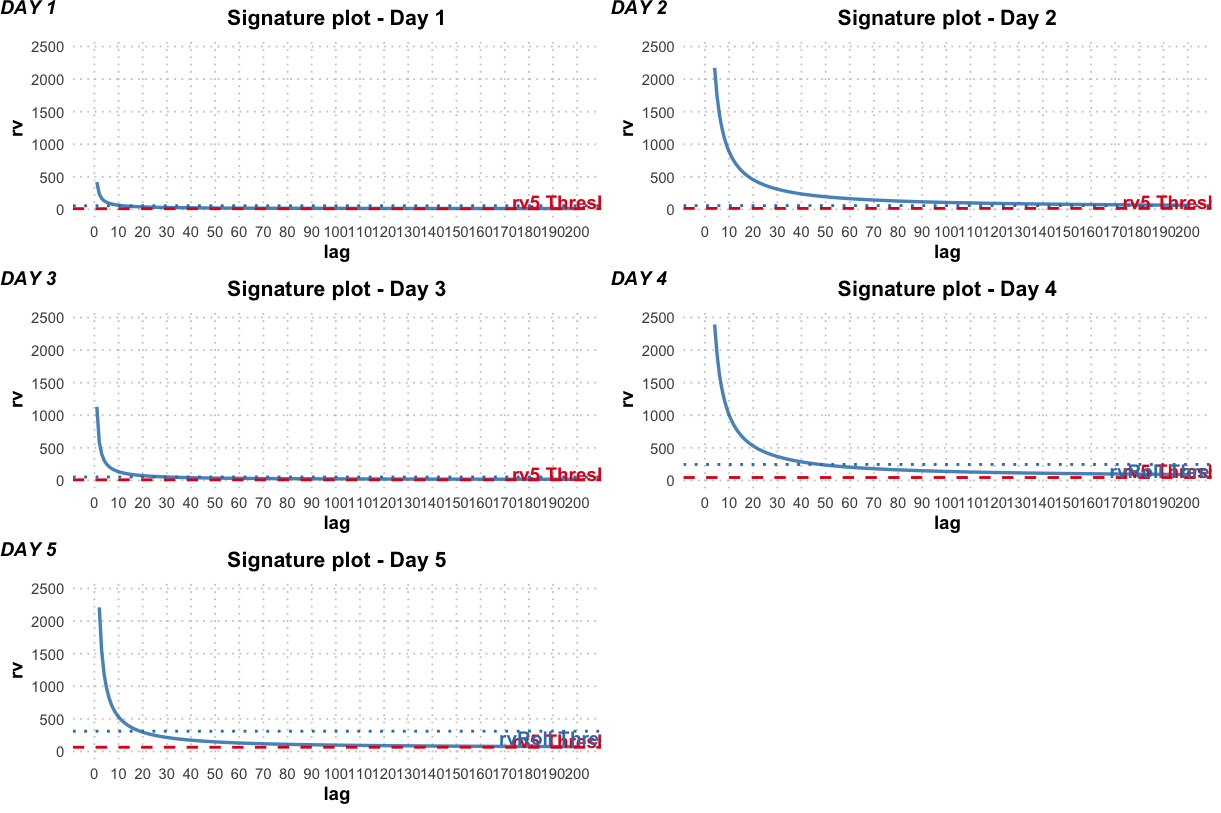
\includegraphics[width=0.8\textwidth]{volatility_signature_plot.png}
\end{adjustbox}
\caption{Signature plot}
\label{fig:S}
\end{figure}



\begin{figure}[H]
\centering
\begin{adjustbox}{max width=\textwidth}
    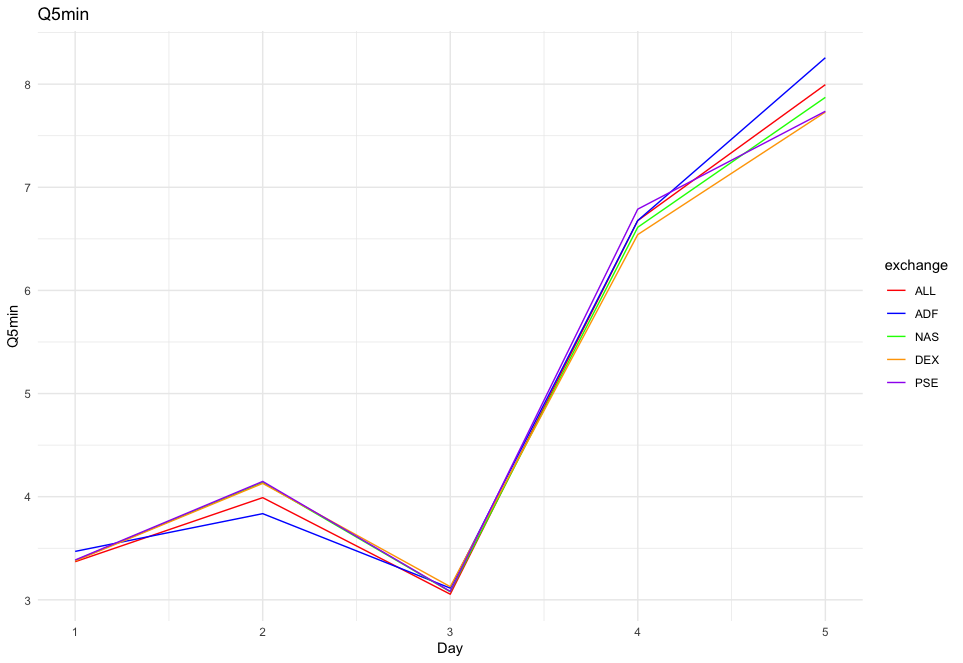
\includegraphics[width=0.8\textwidth]{plot_q5min.png}
\end{adjustbox}
\caption{$q_{5min}\; plot\; across\; exchanges$}
\label{fig:q_5min_plot}
\end{figure}




\subsubsection{Roll Model vs Realized Variance}

\begin{table}[H]
\centering
\begin{adjustbox}{width=\textwidth}
\begin{tabular}{lcccccccccc}
\toprule
\textbf{Type} & \multicolumn{2}{c}{\textbf{ALL}} & \multicolumn{2}{c}{\textbf{ADF}} & \multicolumn{2}{c}{\textbf{NAS}} & \multicolumn{2}{c}{\textbf{DEX}} & \multicolumn{2}{c}{\textbf{PSE}} \\
\cmidrule(lr){2-3} \cmidrule(lr){4-5} \cmidrule(lr){6-7} \cmidrule(lr){8-9} \cmidrule(lr){10-11}
 & rv(q) & $\sigma$ & rv(q) & $\sigma$ & rv(q) & $\sigma$ & rv(q) & $\sigma$ & rv(q) & $\sigma$ \\
\midrule
$q_1$       & 419.49 & 20.48 & 388.19 & 19.70 & 11.33 & 3.37  & 11.22 & 3.35  & 10.79 & 3.28  \\
$q_2$       & 237.95 & 15.43 & 217.78 & 14.76 & 11.33 & 3.37  & 10.62 & 3.26  & 10.70 & 3.27  \\
$q_{5min}$   & 11.35  & 3.37  & 12.04  & 3.47  & 11.43 & 3.38  & 11.40 & 3.38  & 11.47 & 3.39  \\
\midrule
& {$rv_{Roll}$} & {$\sigma_{day}^{roll}$} & {$rv_{Roll}$} & {$\sigma_{day}^{roll}$} & {$rv_{Roll}$} & {$\sigma_{day}^{roll}$}& {$rv_{Roll}$} & {$\sigma_{day}^{roll}$}& {$rv_{Roll}$} & {$\sigma_{day}^{roll}$} \\
Roll model & 56.40  & 7.51  & 47.37  & 6.88  & 10.98 & 3.31  & 10.01 & 3.16  & 10.63 & 3.26  \\
Trades     & \multicolumn{2}{c}{758112} & \multicolumn{2}{c}{483079} & \multicolumn{2}{c}{124082} & \multicolumn{2}{c}{64315} & \multicolumn{2}{c}{38855} \\
\bottomrule
\end{tabular}
\end{adjustbox}
\caption{Day 1}
\label{tab:summary_table}
\end{table}


\begin{table}[h!]
\centering
\begin{adjustbox}{width=\textwidth}
\begin{tabular}{lcccccccccc}
\toprule
\textbf{Type} & \multicolumn{2}{c}{\textbf{ALL}} & \multicolumn{2}{c}{\textbf{ADF}} & \multicolumn{2}{c}{\textbf{NAS}} & \multicolumn{2}{c}{\textbf{DEX}} & \multicolumn{2}{c}{\textbf{PSE}} \\
\cmidrule(lr){2-3} \cmidrule(lr){4-5} \cmidrule(lr){6-7} \cmidrule(lr){8-9} \cmidrule(lr){10-11}
 & rv(q) & $\sigma$ & rv(q) & $\sigma$ & rv(q) & $\sigma$ & rv(q) & $\sigma$ & rv(q) & $\sigma$ \\
\midrule
$q_1$       & 8547.23 & 92.45 & 8474.62 & 92.06 & 24.18 & 4.92  & 21.94 & 4.68  & 21.13 & 4.60  \\
$q_2$        & 4302.79 & 65.60 & 4258.68 & 65.26 & 22.83 & 4.78  & 20.84 & 4.56  & 20.85 & 4.57  \\
$q_{5min}$   & 15.92  & 3.99  & 14.71  & 3.84  & 17.12 & 4.14  & 17.05 & 4.13  & 17.21 & 4.15  \\
\midrule
& {$rv_{Roll}$} & {$\sigma_{day}^{roll}$} & {$rv_{Roll}$} & {$\sigma_{day}^{roll}$} & {$rv_{Roll}$} & {$\sigma_{day}^{roll}$}& {$rv_{Roll}$} & {$\sigma_{day}^{roll}$}& {$rv_{Roll}$} & {$\sigma_{day}^{roll}$} \\
Roll model & 58.34  & 7.64  & 42.75  & 6.88  & 21.51 & 4.64  & 19.74 & 4.44  & 20.56 & 4.53  \\
Trades     & \multicolumn{2}{c}{1373398} & \multicolumn{2}{c}{833862} & \multicolumn{2}{c}{240038} & \multicolumn{2}{c}{112176} & \multicolumn{2}{c}{87602} \\
\bottomrule
\end{tabular}
\end{adjustbox}
\caption{Day 2}
\label{tab:updated_summary_table}
\end{table}


\begin{table}[h!]
\centering
\begin{adjustbox}{width=\textwidth}
\begin{tabular}{lcccccccccc}
\toprule
\textbf{Type} & \multicolumn{2}{c}{\textbf{ALL}} & \multicolumn{2}{c}{\textbf{ADF}} & \multicolumn{2}{c}{\textbf{NAS}} & \multicolumn{2}{c}{\textbf{DEX}} & \multicolumn{2}{c}{\textbf{PSE}} \\
\cmidrule(lr){2-3} \cmidrule(lr){4-5} \cmidrule(lr){6-7} \cmidrule(lr){8-9} \cmidrule(lr){10-11}
 & rv(q) & $\sigma$ & rv(q) & $\sigma$ & rv(q) & $\sigma$ & rv(q) & $\sigma$ & rv(q) & $\sigma$ \\
\midrule
$q_1$        & 1130.13 & 33.62 & 1101.57 & 33.19 & 11.83 & 3.44 & 11.32 & 3.37 & 10.66 & 3.26 \\
$q_2$       & 591.30  & 24.32 & 573.52  & 23.95 & 11.36 & 3.37 & 10.92 & 3.30 & 10.73 & 3.28 \\
$q_{5min}$   & 9.33    & 3.05  & 9.69    & 3.11  & 9.48  & 3.08 & 9.78  & 3.13 & 9.50  & 3.08 \\
\midrule
& {$rv_{Roll}$} & {$\sigma_{day}^{roll}$} & {$rv_{Roll}$} & {$\sigma_{day}^{roll}$} & {$rv_{Roll}$} & {$\sigma_{day}^{roll}$}& {$rv_{Roll}$} & {$\sigma_{day}^{roll}$}& {$rv_{Roll}$} & {$\sigma_{day}^{roll}$} \\
Roll model & 52.47  & 7.24  & 45.48  & 6.88  & 10.90 & 3.30 & 10.51 & 3.24 & 10.81 & 3.29 \\
Trades     & \multicolumn{2}{c}{833824} & \multicolumn{2}{c}{493149} & \multicolumn{2}{c}{148489} & \multicolumn{2}{c}{69071} & \multicolumn{2}{c}{60175} \\
\bottomrule
\end{tabular}
\end{adjustbox}
\caption{Day 3}
\label{tab:final_summary_table}
\end{table}

\begin{table}[H]
\centering
\begin{adjustbox}{width=\textwidth}
\begin{tabular}{lcccccccccc}
\toprule
\textbf{Type} & \multicolumn{2}{c}{\textbf{ALL}} & \multicolumn{2}{c}{\textbf{ADF}} & \multicolumn{2}{c}{\textbf{NAS}} & \multicolumn{2}{c}{\textbf{DEX}} & \multicolumn{2}{c}{\textbf{PSE}} \\
\cmidrule(lr){2-3} \cmidrule(lr){4-5} \cmidrule(lr){6-7} \cmidrule(lr){8-9} \cmidrule(lr){10-11}
 & rv(q) & $\sigma$ & rv(q) & $\sigma$ & rv(q) & $\sigma$ & rv(q) & $\sigma$ & rv(q) & $\sigma$ \\
\midrule
$q_1$       & 9031.90 & 95.04 & 8744.54 & 93.51 & 69.02 & 8.31 & 60.87 & 7.80 & 53.72 & 7.33 \\
$q_2$       & 4638.52 & 68.11 & 4486.54 & 66.98 & 63.15 & 7.95 & 54.28 & 7.37 & 51.55 & 7.18 \\
$q_{5min}$   & 44.59   & 6.68  & 44.59   & 6.68  & 43.73 & 6.61 & 42.79 & 6.54 & 46.08 & 6.79 \\
\midrule
& {$rv_{Roll}$} & {$\sigma_{day}^{roll}$} & {$rv_{Roll}$} & {$\sigma_{day}^{roll}$} & {$rv_{Roll}$} & {$\sigma_{day}^{roll}$}& {$rv_{Roll}$} & {$\sigma_{day}^{roll}$}& {$rv_{Roll}$} & {$\sigma_{day}^{roll}$} \\
Roll model & 245.14  & 15.66 & 228.55  & 6.88  & 57.28 & 7.57 & 47.68 & 6.90 & 49.38 & 7.03 \\
Trades     & \multicolumn{2}{c}{2313397} & \multicolumn{2}{c}{1129191} & \multicolumn{2}{c}{483448} & \multicolumn{2}{c}{257414} & \multicolumn{2}{c}{182361} \\
\bottomrule
\end{tabular}
\end{adjustbox}
\caption{Day 4}
\label{tab:latest_summary_table}
\end{table}


\begin{table}[H]
\centering
\begin{adjustbox}{width=\textwidth}
\begin{tabular}{lcccccccccc}
\toprule
\textbf{Type} & \multicolumn{2}{c}{\textbf{ALL}} & \multicolumn{2}{c}{\textbf{ADF}} & \multicolumn{2}{c}{\textbf{NAS}} & \multicolumn{2}{c}{\textbf{DEX}} & \multicolumn{2}{c}{\textbf{PSE}} \\
\cmidrule(lr){2-3} \cmidrule(lr){4-5} \cmidrule(lr){6-7} \cmidrule(lr){8-9} \cmidrule(lr){10-11}
 & rv(q) & $\sigma$ & rv(q) & $\sigma$ & rv(q) & $\sigma$ & rv(q) & $\sigma$ & rv(q) & $\sigma$ \\
\midrule
$q_1$       & 4111.19 & 64.12 & 3926.35 & 62.66 & 62.96 & 7.93 & 59.66 & 7.72 & 52.17 & 7.22 \\
$q_2$       & 2210.60 & 47.02 & 3926.35 & 62.66 & 59.32 & 7.70 & 54.33 & 7.37 & 51.74 & 7.19 \\
$q_{5min}$   & 63.92   & 8.00  & 68.16   & 8.26  & 61.97 & 7.87 & 59.75 & 7.73 & 59.86 & 7.74 \\
\midrule
& {$rv_{Roll}$} & {$\sigma_{day}^{roll}$} & {$rv_{Roll}$} & {$\sigma_{day}^{roll}$} & {$rv_{Roll}$} & {$\sigma_{day}^{roll}$}& {$rv_{Roll}$} & {$\sigma_{day}^{roll}$}& {$rv_{Roll}$} & {$\sigma_{day}^{roll}$} \\
Roll model & 310.03  & 17.61 & 246.24  & 15.69 & 55.69 & 7.46 & 48.99 & 7.00 & 51.31 & 7.16 \\
Trades     & \multicolumn{2}{c}{1777544} & \multicolumn{2}{c}{949185} & \multicolumn{2}{c}{336278} & \multicolumn{2}{c}{203923} & \multicolumn{2}{c}{116282} \\
\bottomrule
\end{tabular}
\end{adjustbox}
\caption{Day 5}
\label{tab:latest_summary_table}
\end{table}

\section{PIN measure}

\end{document}
